\section{Sicherheit}

\paragraph{Übersicht}
\begin{items}
  \item \textbf{Bausteine}: Signatur, Verschlüsselung, Hashfunktion, Message Authentication Code, Schlüsselaustausch,...
  \item \textbf{Schutzziele}: Vertraulichkeit, Integrität, Authentizität, Privatheit, (Nicht)-Abstreitbarkeit,...
  \item \textbf{Angriffe}: Abhören, Einfügen, Manipulieren, Man in the Middle, Replay, Denial of Service,...
  \item \textbf{System/Protokoll}: TLS/SSL, IPsec, Kerberos,...
  \item \( \leadsto \) \textbf{System/Protokoll} verwendet \textbf{Bausteine} um \textbf{Schutzziele} zu realisieren und vor \\* \phantom{.} \textbf{Angriffen} zu schützen
\end{items}

\paragraph{Schutzziele}
\begin{items}
  \item \emph{Anforderungen an eine Komponente oder ein System, die erfüllt werden müssen, um schützenswerte Güter vor Bedrohen zu schützen}
  \item \textbf{Kategorien}: \\*
    - \textbf{C}onfidentiality \\*
    - \textbf{I}ntegrity \\*
    - \textbf{A}vailability
  \item weitere Schutzziele: \\*
    - Authentizität \\*
    - Privatheit \\*
    - (Nicht-)Abstreitbarkeit
\end{items}

\paragraph{Schutzziele --- Vertraulichkeit}
\begin{items}
  \item \emph{Ein System bewart Vertraulichkeit, wenn es keine unauthorisierte Informationsgewinnung ermöglicht}
  \item \textbf{Bausteine}: (A)-Symmetrische Verschlüsselung
\end{items}

\paragraph{Schutzziele --- Integrität}
\begin{items}
  \item \textbf{starke Integrität}: \emph{Ein System bewahrt starke Integrität, wenn es nicht möglich ist, Daten unauthorisiert zu manipulieren}
  \item \textbf{schwache Integrität}: \emph{Ein System bewahrt schwache Integrität, wenn unauthorisierte Manipulationen an Daten nicht unbemerkt möglich sind}
  \item \textbf{Bausteine}: Tamper Proof-Module, Message Authentication Codes (MAC)
  \item \textbf{Probleme}: \\*
    - Manipulationen in vielen Fällen nicht zu verhindern \\*
    \( \leadsto \) wenigstens nicht unbemerkt \( \leadsto \) \textbf{schwache Integrität}
  \item \textbf{Angriffe}: Ersetzen, Einfügen oder Löschen von Daten
\end{items}

\paragraph{Schutzziele --- Authentizität}
\begin{items}
  \item \emph{Die angegebene Datenquelle ist tatsächliche Quelle} + Datenintegrität
  \item \textbf{Subjektechtheit}: Bob will sicherstellen, dass er tatsächlich mit Alice kommuniziert \\* \( \leadsto \) \textbf{Authentifikation}
  \item \textbf{Datenechtheit}: Bob will sicherstellen, dasss Daten tatsächlich von Alice sind
  \item \textbf{Bausteine}: Zertifikate, Signaturen, gemeinsames Geheimnis
\end{items}

\paragraph{Schutzziele --- Verfügbarkeit}
\begin{items}
  \item \emph{Beschreibt, in welchem Maße die Systemfunktionalität von berechtigen Subjekten unabhängig von Einflüssen in Anspruch genommen werden kann}
\end{items}

\paragraph{Angriffe}
\begin{items}
  \item Sniffing, Denial of Service,\dots
\end{items}

\paragraph{Bausteine}
\begin{items}
  \item \textbf{Verschlüsselung}: \\*
    - \textbf{symmetrisch}: Ent- und Verschlüsseln mit einem Schlüssel, sehr effizient \\*
    - \textbf{asymmetrisch}: Verschlüsseln: öffentlicher Schlüssel, Entschlüsseln: privater
  \item \textbf{Integritätssicherung}: \\*
    - \textbf{kryptografische Hashfunktion}: verwendet symmetrische Kryptografie \\*
    - \textbf{digitale Signatur}: verwendet asymmetrische Kryptografie
  \item \textbf{Schlüsselaustausch}
  \item \textbf{Message Authentication Code}: \\*
    - Ziel: Empfänger erkennt Manipulation an empfangenen Daten \\*
    - Voraussetzung: Alice und Bob haben gleichen symmetrischen Schlüssel \\*
    - Vorgehensweise: Alice hängt Hash von Nachricht + Schlüssel an Nachricht an
  \item \textbf{Digitale Signatur}: \\*
    - Ziel: Bob kann verifizieren, dass nur Alice nur dieses Dokument unterschrieben hat \\*
    - Vorgehensweise: Hash des Dokuments mit privatem Schlüssel verschlüsseln, als \\* \phantom{-} Signatur mitsenden, entschlüsseln mit öffentlichem Schlüssel
  \item \textbf{Digitales Zertifikat}: \\*
    - Ziel: Verifizieren, dass jemand der ist, für den er sich ausgibt \\*
    - Problem: kann man nicht selbst überprüfen \( \leadsto \) verlassen auf Dritte \\*
    - Vorgehensweise: Überprüfung durch \emph{certificate authority} (CA), \\* \phantom{-} Zertifikat = Authentifikation des öffentlichen Schlüssels
\end{items}

\paragraph{Sicherheitsprotokolle}
\
\begin{figure}[H]\centering\label{Sicherheitsprotokolle}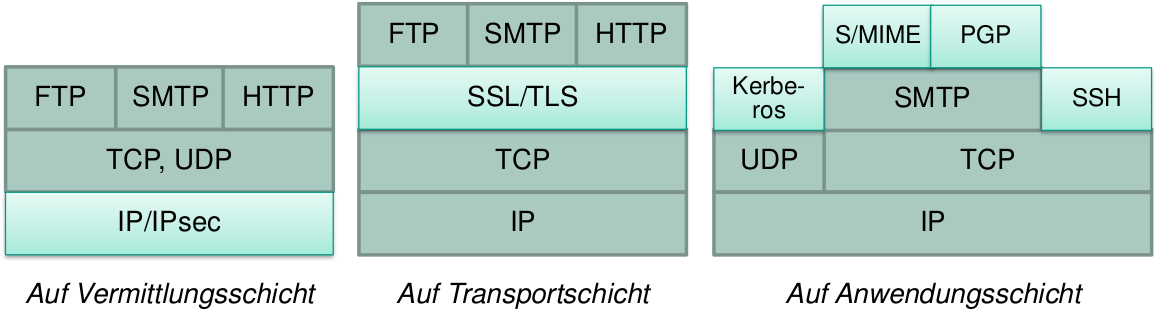
\includegraphics[width=0.33\textwidth]{Sicherheitsprotokolle}\end{figure}